\documentclass{db-practice}

\begin{document}

\title{Ejercicios de paso a tablas}

\section{Compañía aseguradora}

Transforme el siguiente modelo Entidad-Relación en un modelo relacional mediante las reglas del ``\textit{paso a tablas}'':

\begin{figure}[H]
    \centering
    \includegraphics[width=\textwidth]{figs/compañia-aseguradora}
\end{figure}

\section{Tienda de mascotas}

Transforme el siguiente modelo Entidad-Relación en un modelo relacional mediante las reglas del ``\textit{paso a tablas}'':

\begin{figure}[H]
    \centering
    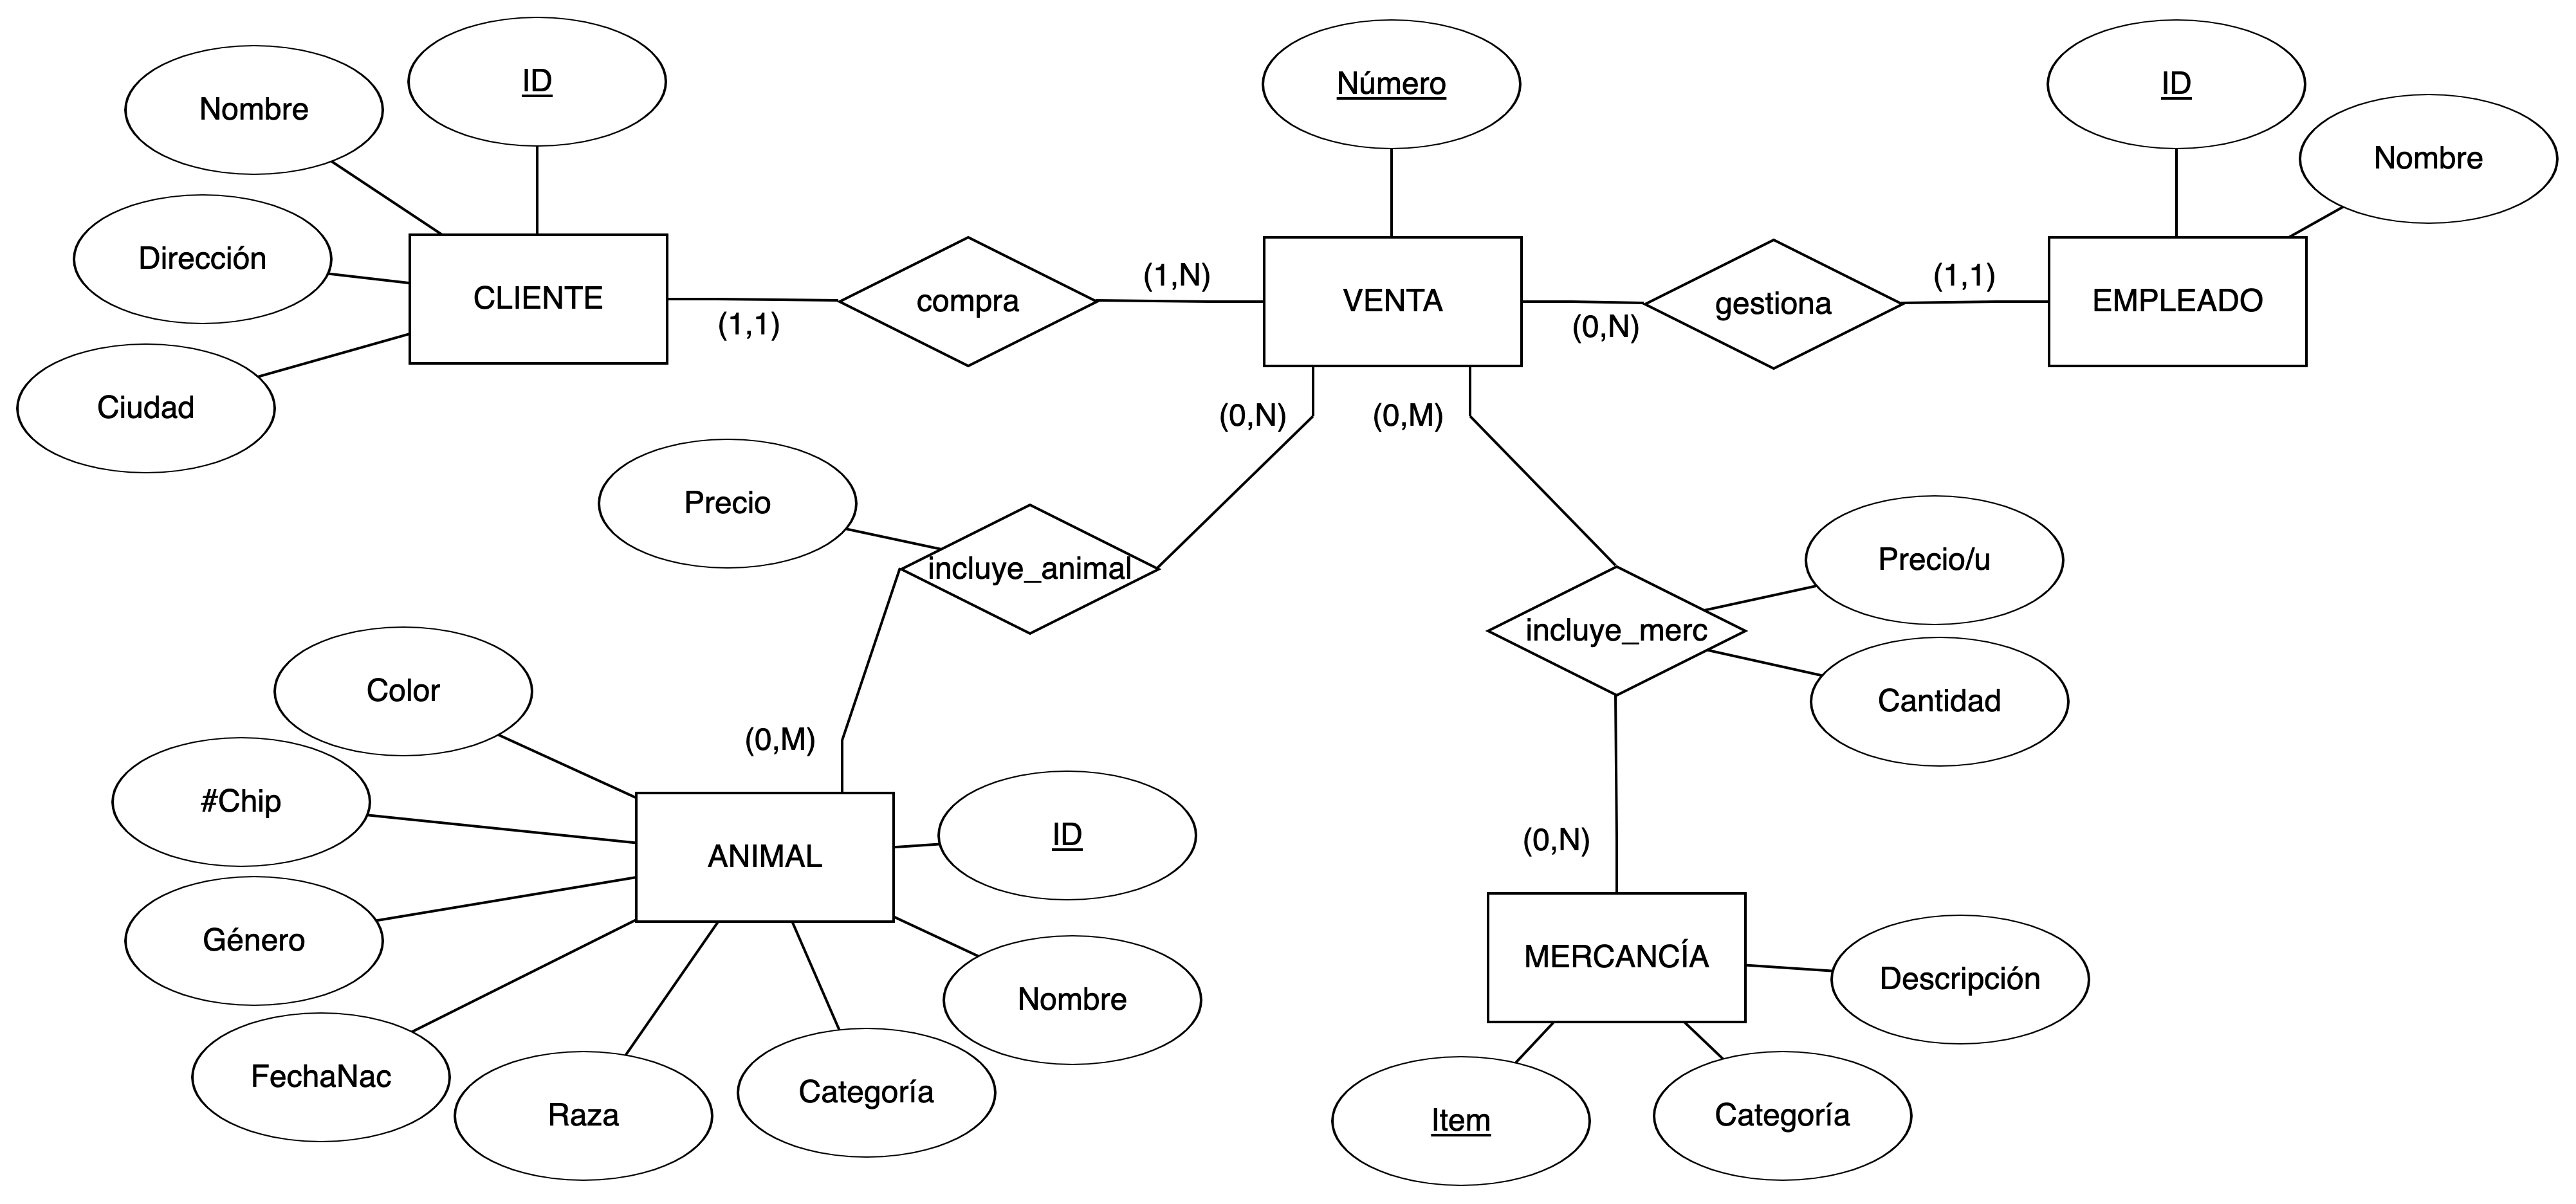
\includegraphics[width=\textwidth]{figs/tienda-de-mascotas}
\end{figure}

\newpage
\section{Permisos de circulación}

Transforme el siguiente modelo Entidad-Relación en un modelo relacional mediante las reglas del ``\textit{paso a tablas}'':

\begin{figure}[H]
    \centering
    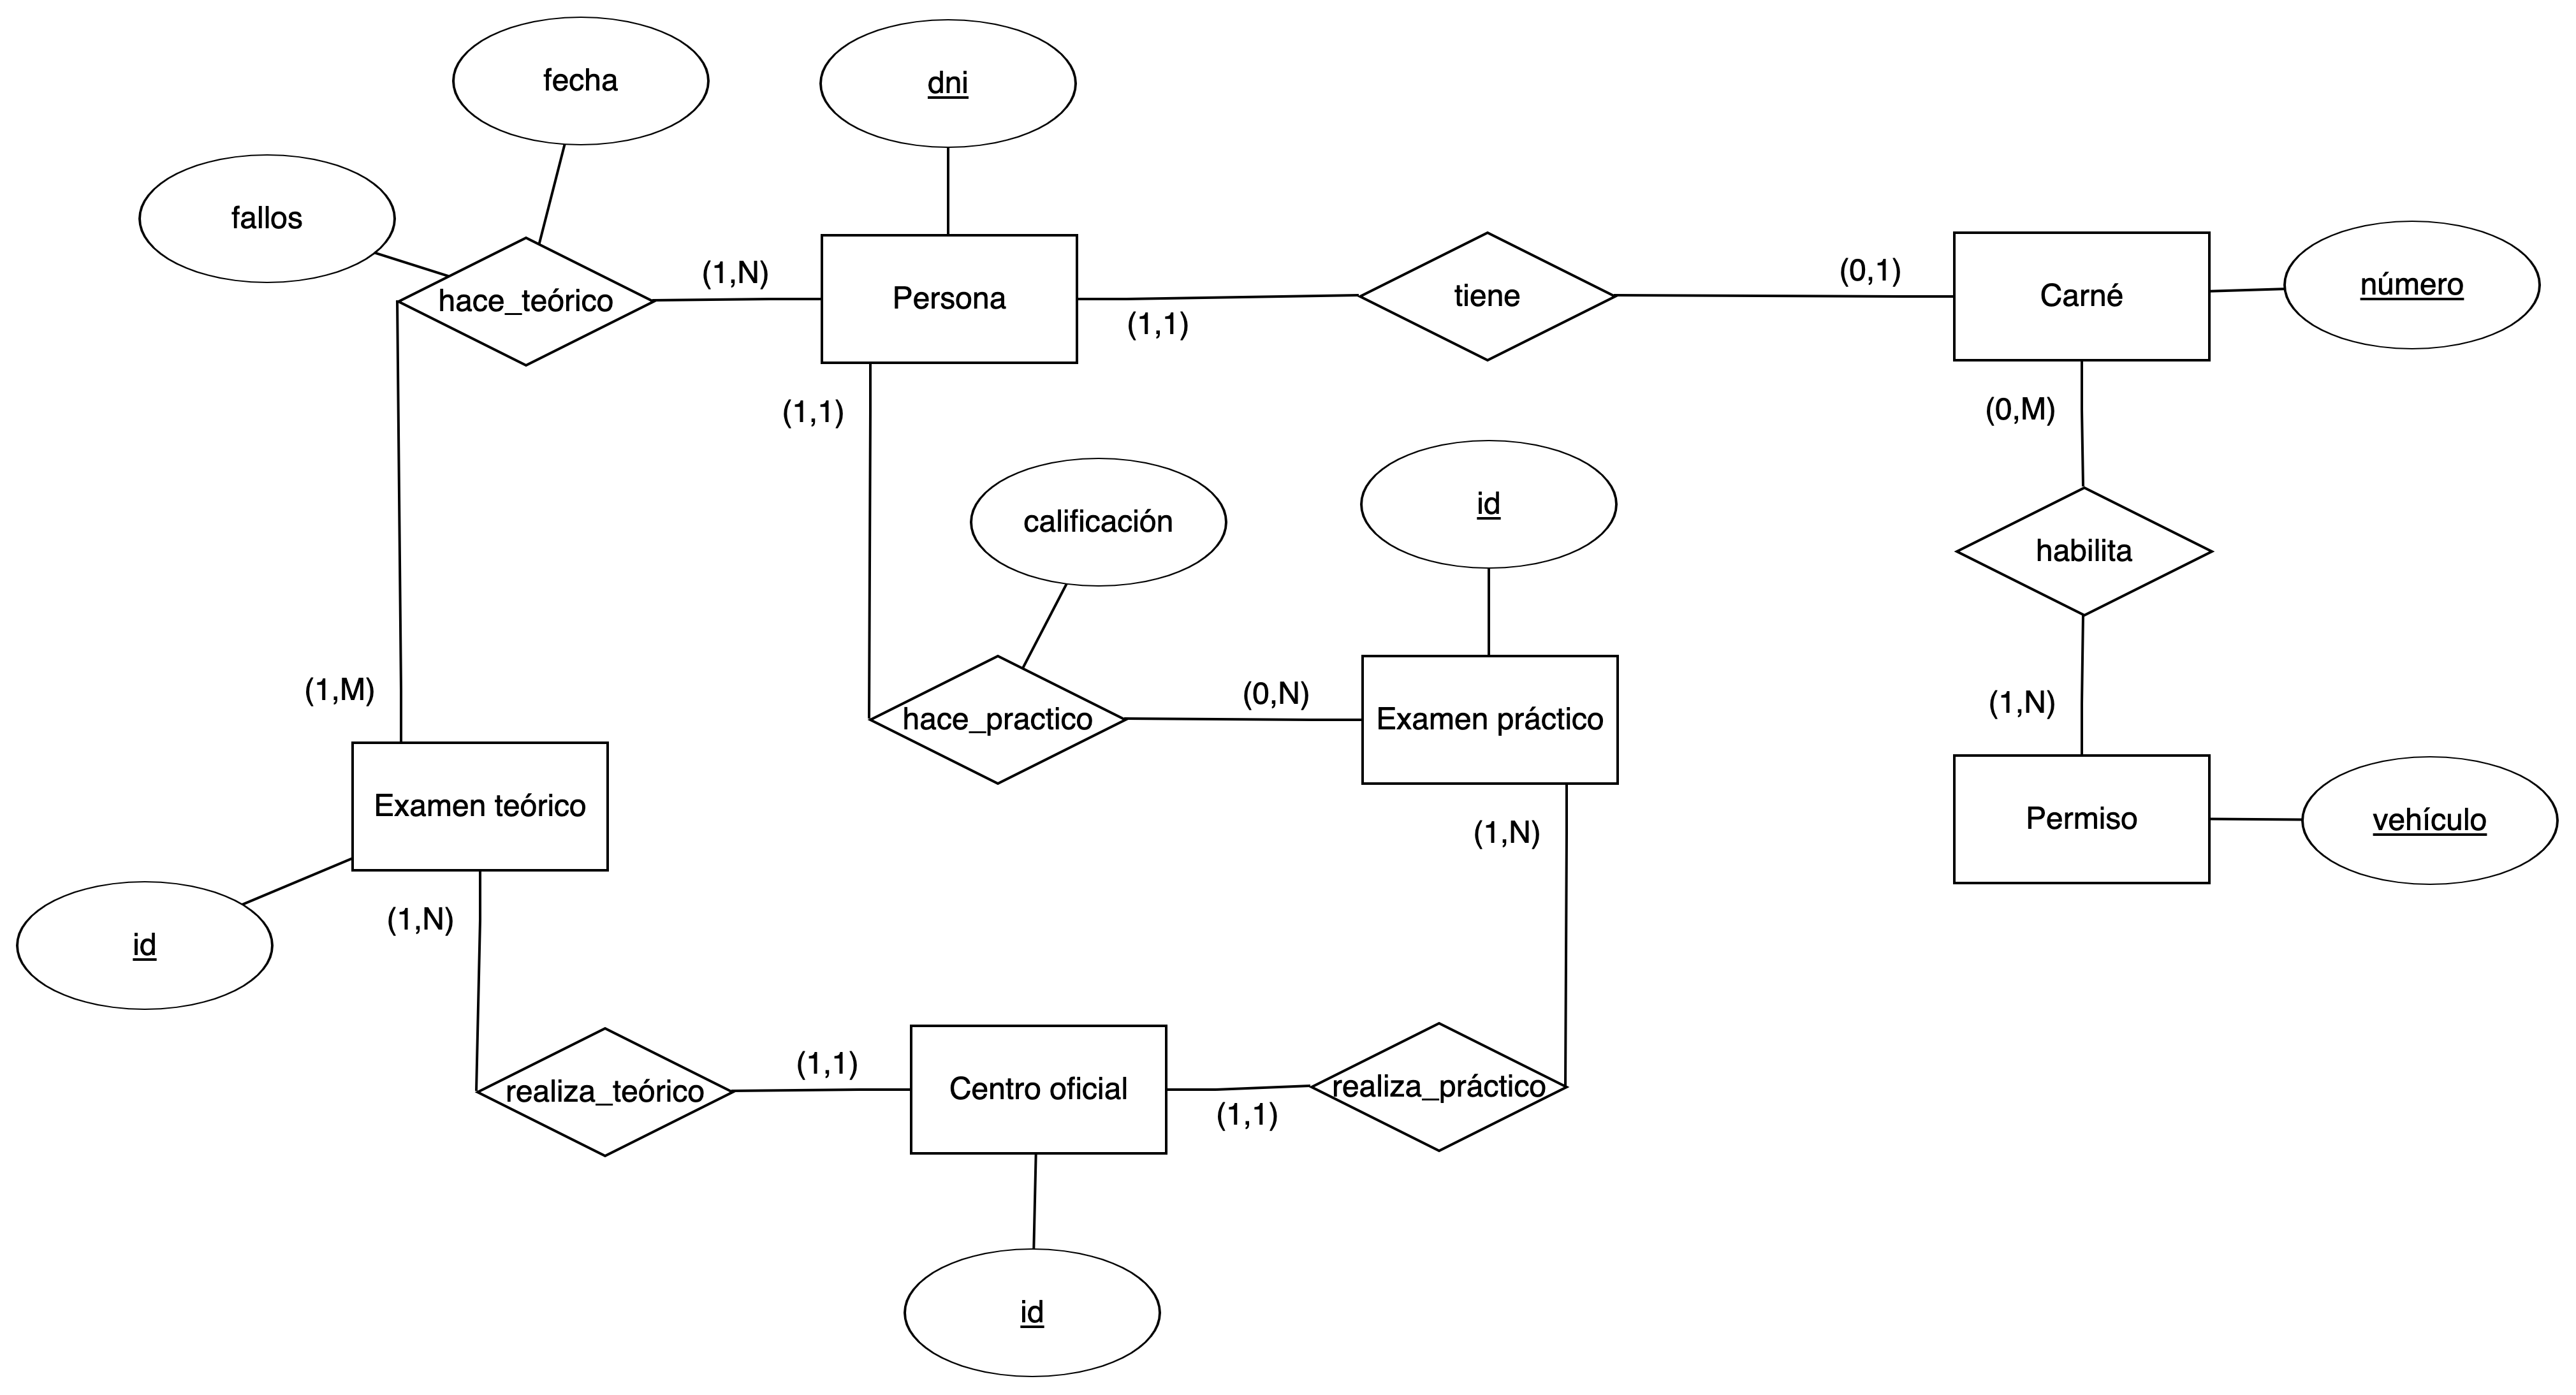
\includegraphics[width=\textwidth]{figs/permiso-de-circulacion}
\end{figure}

\section{Censo de la Unión Europea}

Transforme el siguiente modelo Entidad-Relación en un modelo relacional mediante las reglas del ``\textit{paso a tablas}'':

\begin{figure}[H]
    \centering
    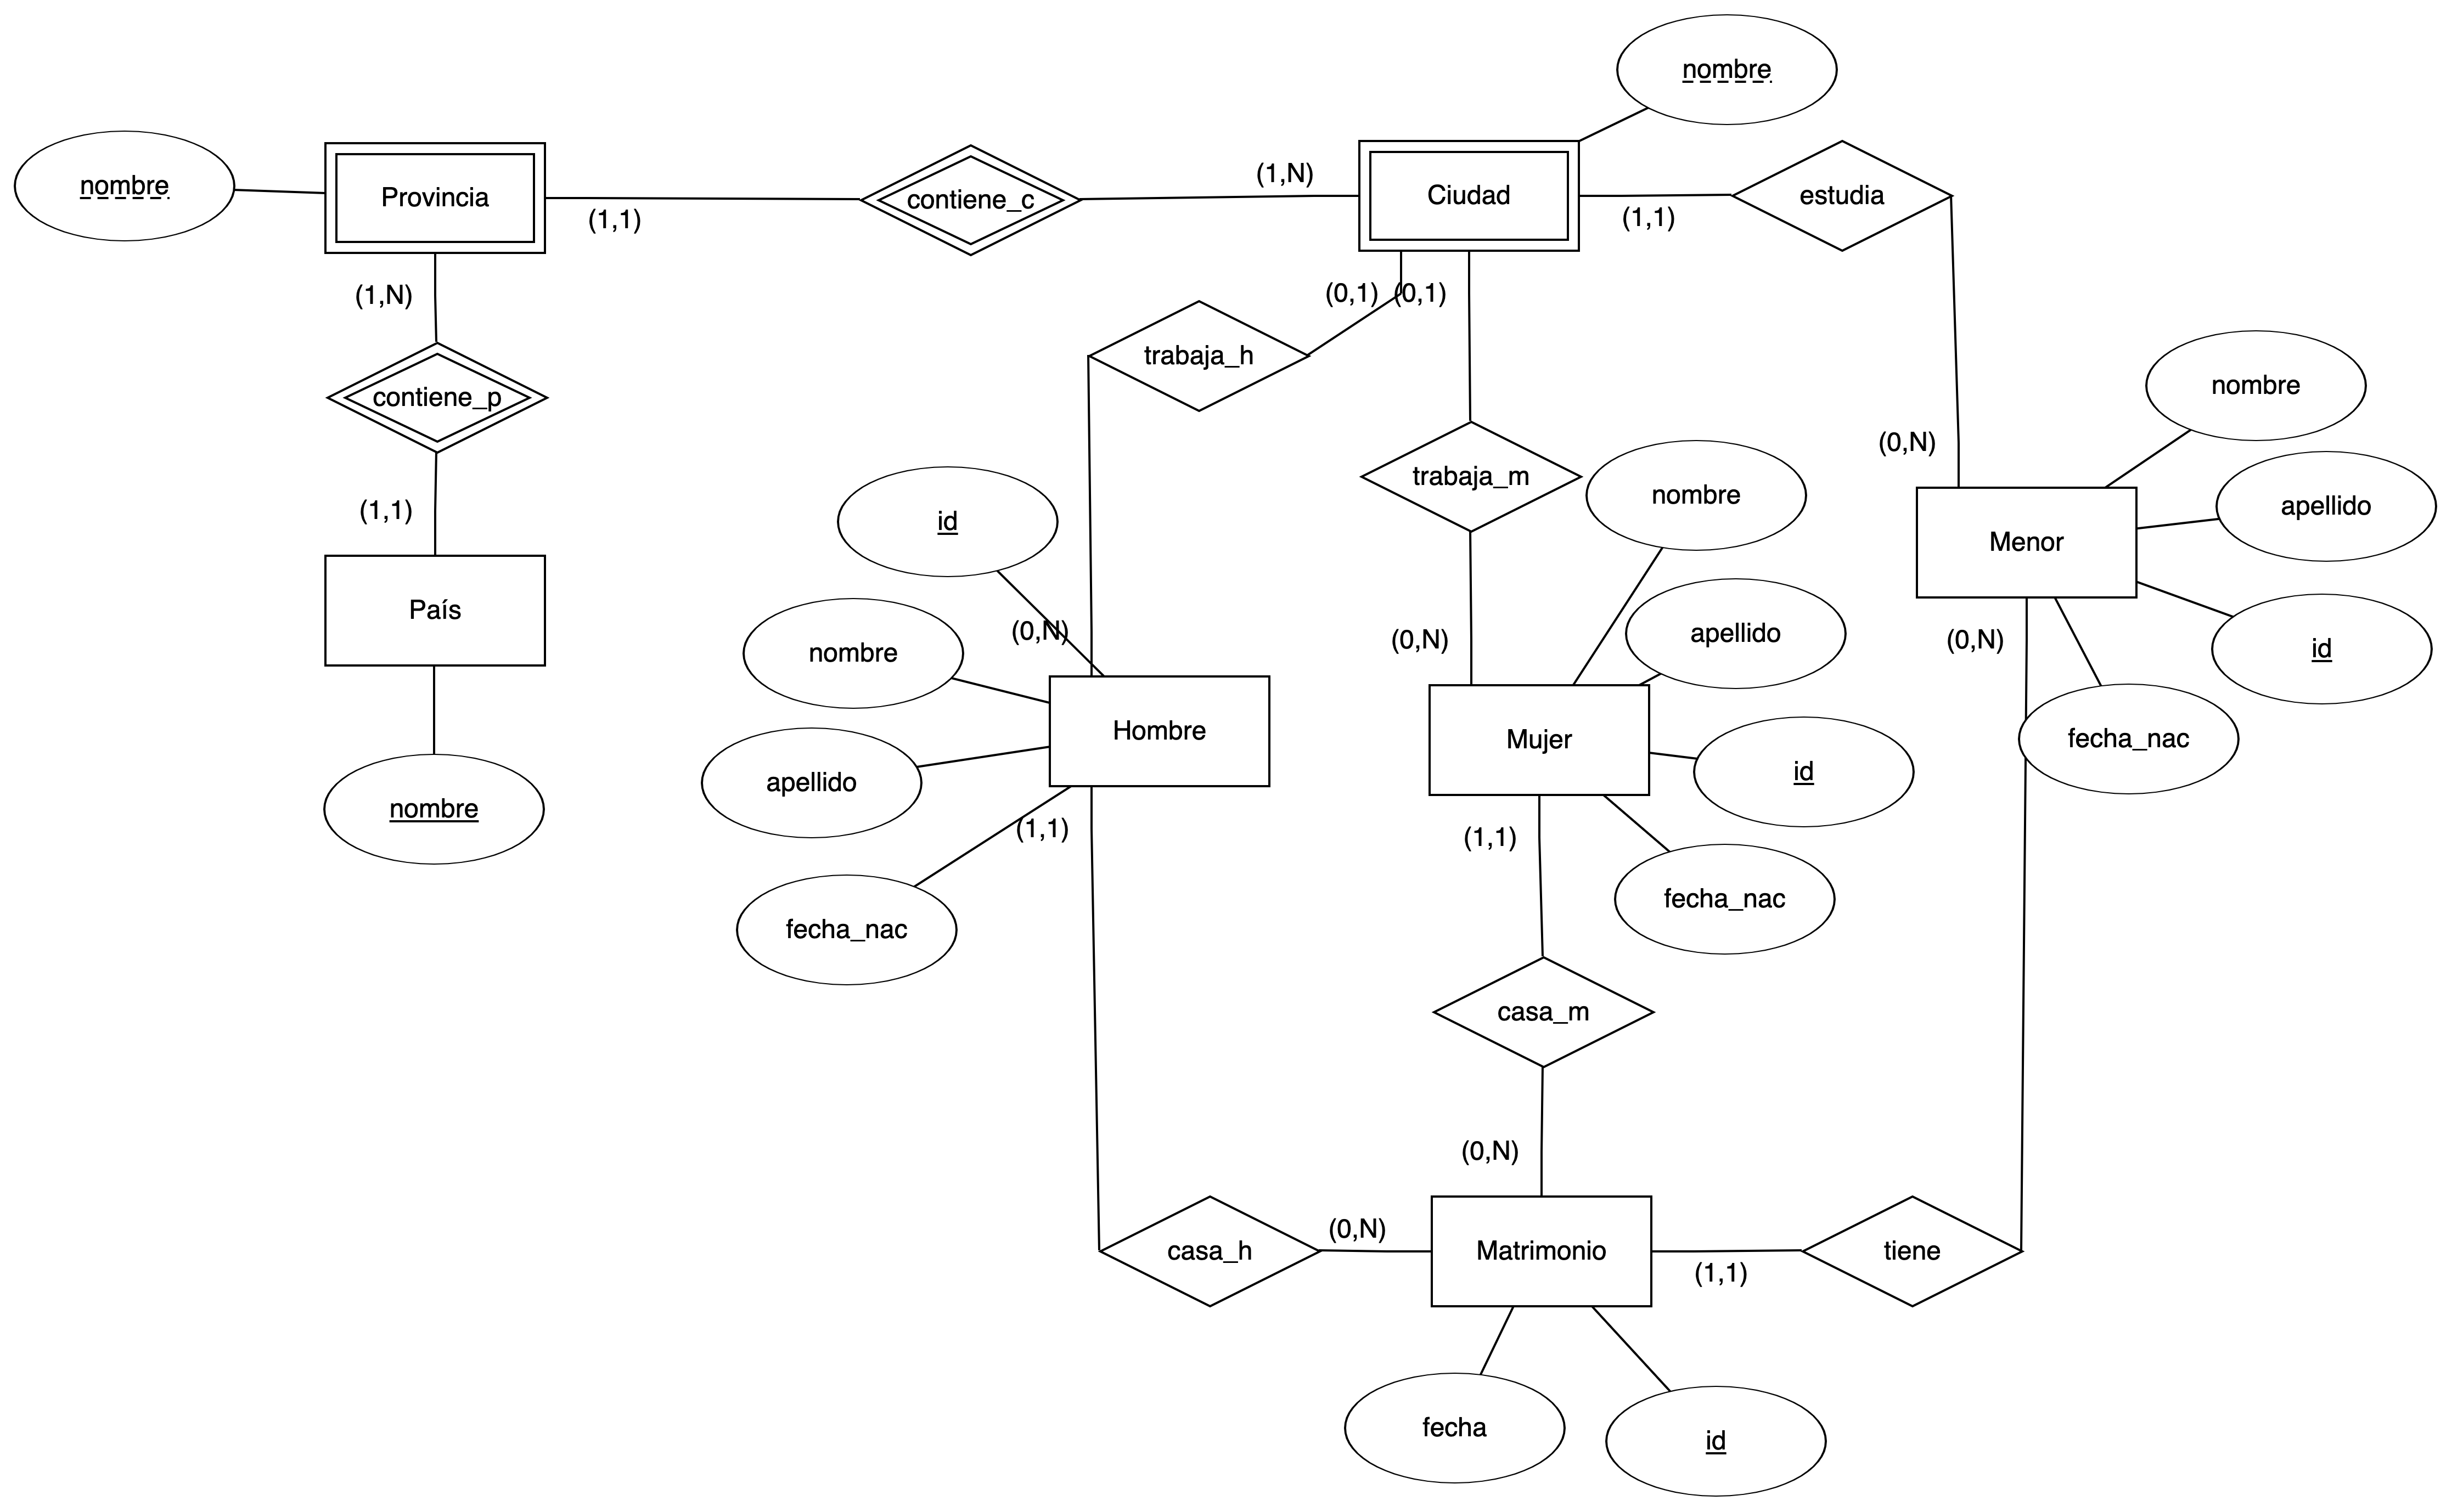
\includegraphics[width=.9\textwidth]{figs/censo-union-europea}
\end{figure}

\section{Desarrollo dirigidos por modelos}

Transforme el siguiente modelo Entidad-Relación en un modelo relacional mediante las reglas del ``\textit{paso a tablas}'':

\begin{figure}[H]
    \centering
    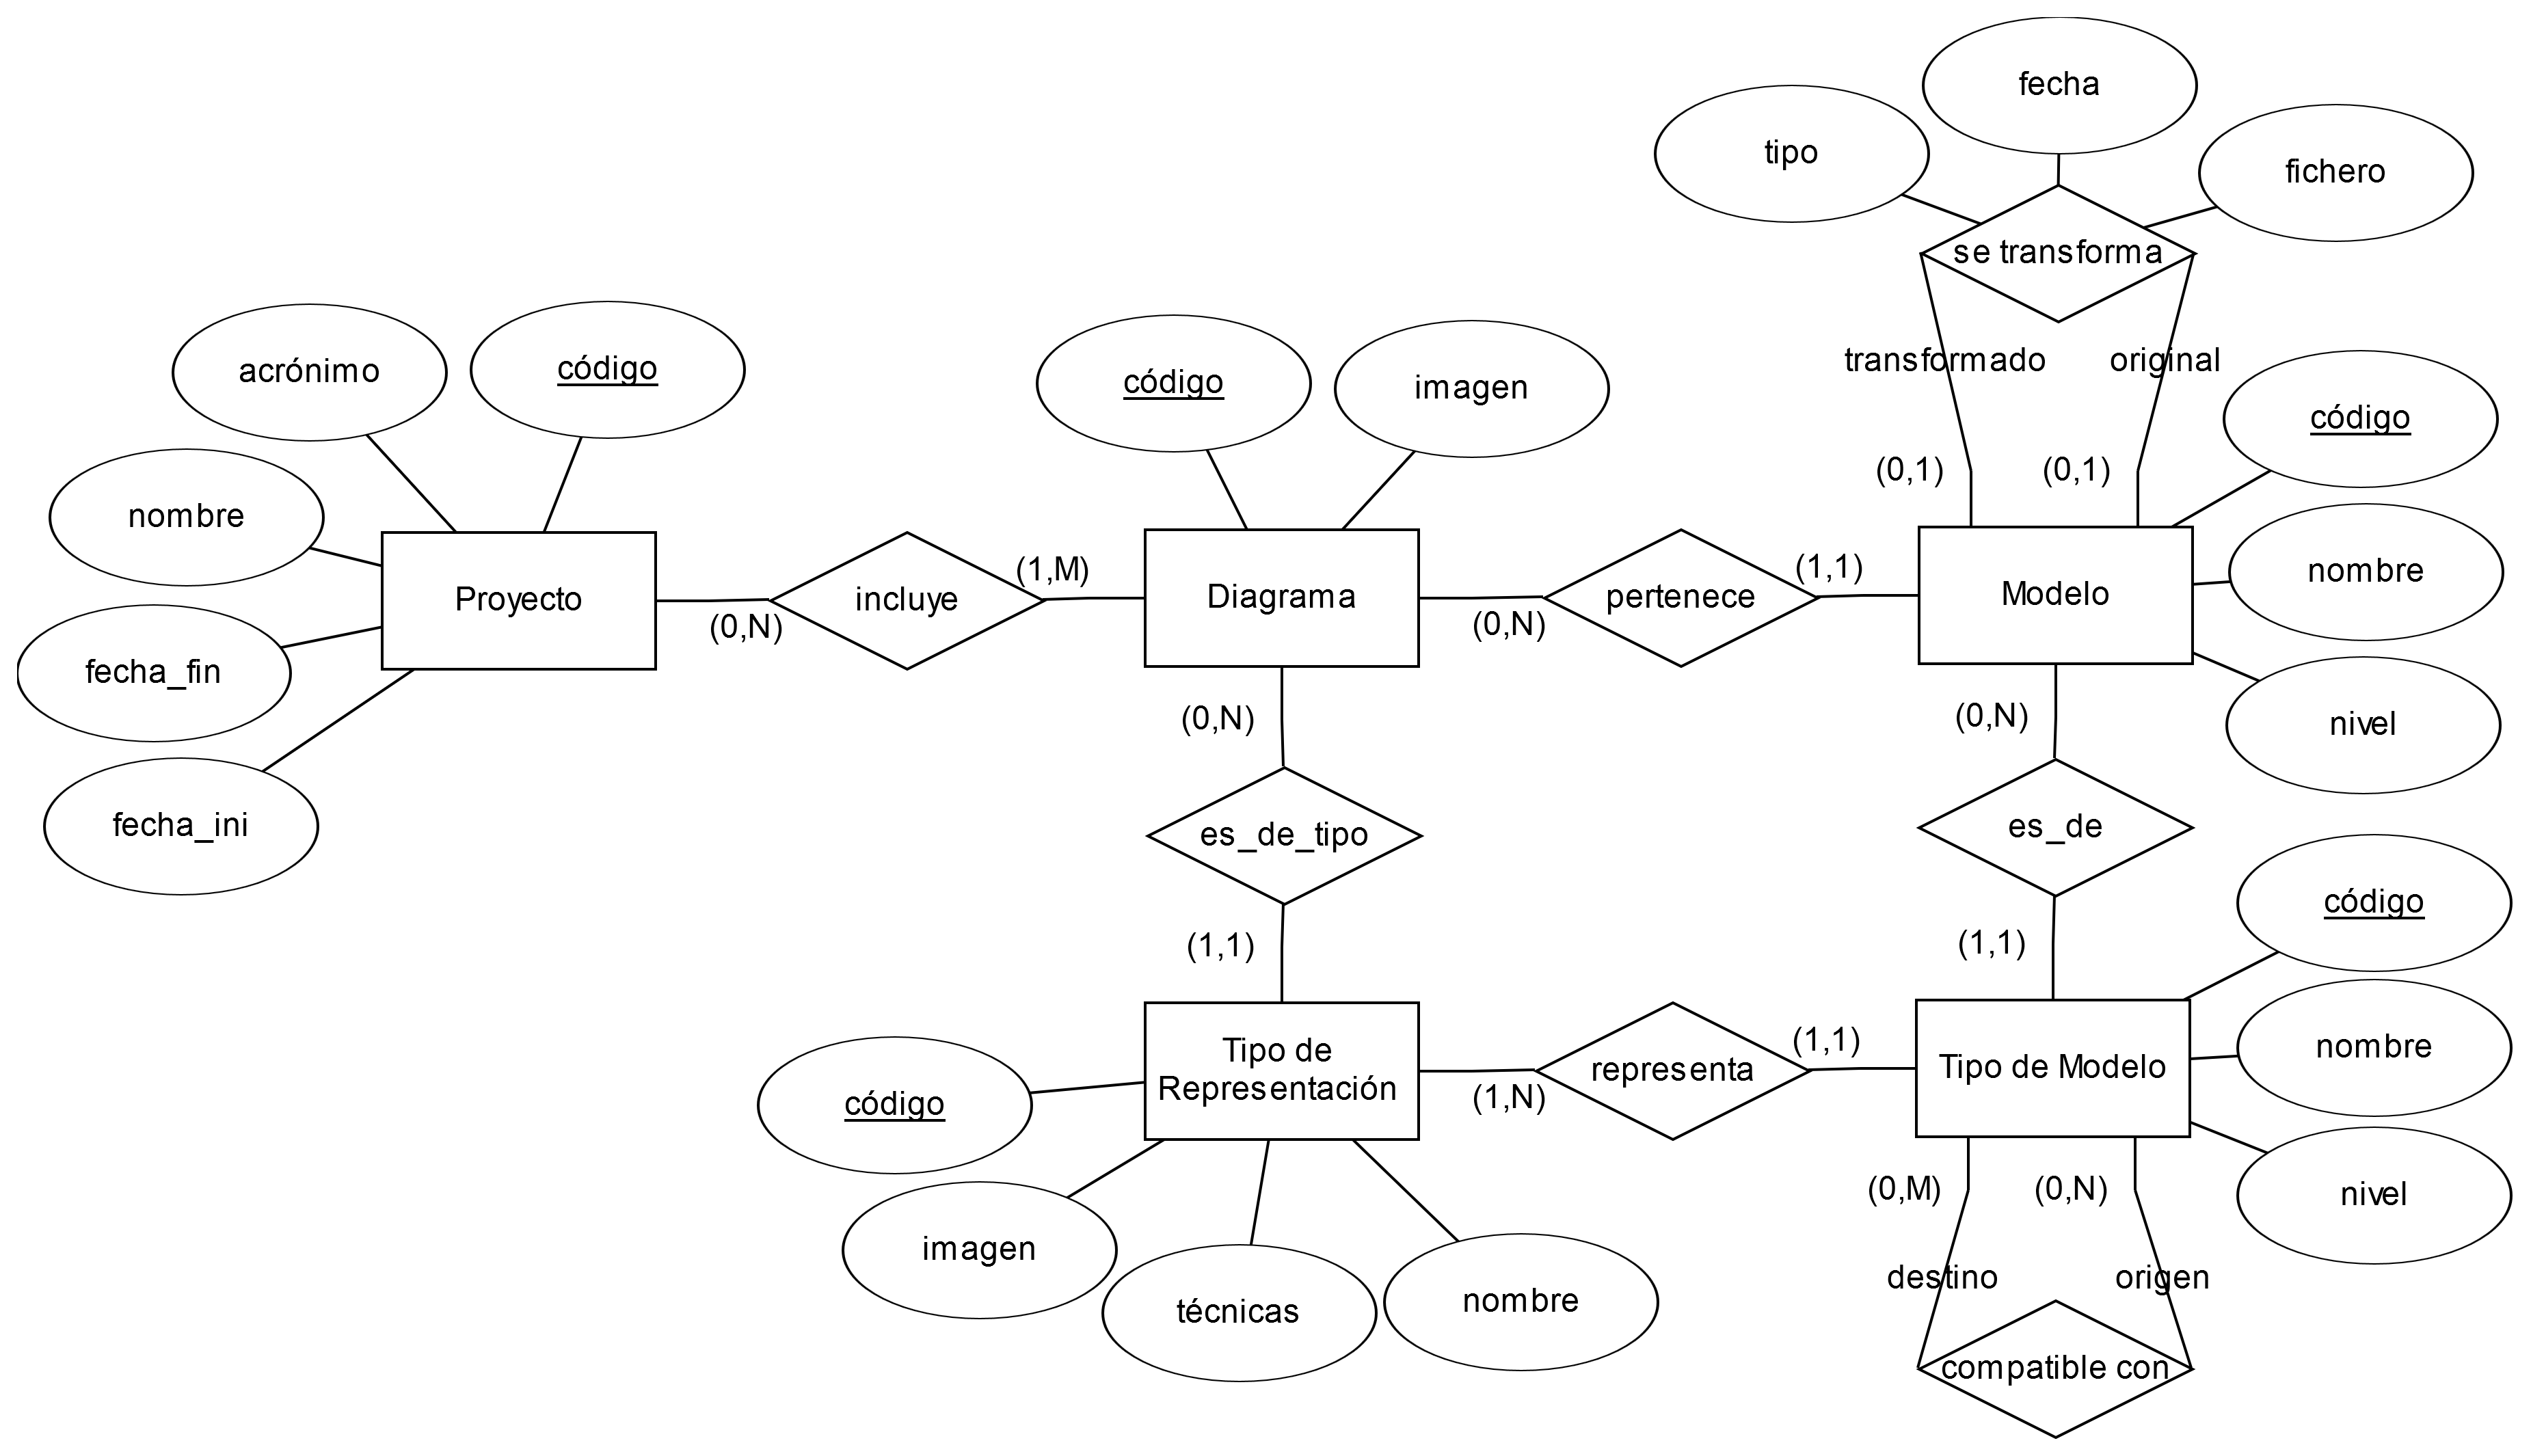
\includegraphics[width=\textwidth]{figs/desarrollo-dirigido-por-modelos}
\end{figure}

\section{Gestión de locales nocturnos}

Transforme el siguiente modelo Entidad-Relación en un modelo relacional mediante las reglas del ``\textit{paso a tablas}'':

\begin{figure}[H]
    \centering
    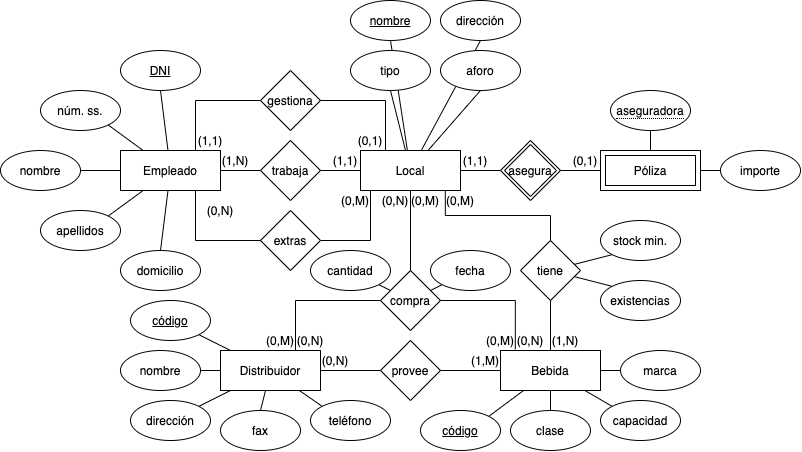
\includegraphics[width=\textwidth]{figs/gestion-locales-nocturnos}
\end{figure}

\end{document}
